\documentclass[12pt]{article}


\usepackage[utf8]{inputenc}
\usepackage{cite}
\usepackage{algorithm}
\usepackage{amsmath}
\usepackage{algpseudocode}
\usepackage{lmodern}
\usepackage{microtype}
\usepackage{amsmath}
\usepackage{mathrsfs}
\usepackage{mathtools}
\usepackage{xcolor}
\usepackage{ulem}
\usepackage{graphicx}
\usepackage{float}
\usepackage{subfigure}
\usepackage[hyphens]{url}
\usepackage{setspace}
\usepackage{titlesec}
\usepackage[title]{appendix}


%\title{Automatic light dimmer}
\title{%
  \Huge BATTLE-SHIP GAME}
\author{Pena Benafa\\pena.benafa@stud.hshl.de\\Patrick Stephen\\stephen-eteng.patrick@stud.hshl.de\\
  \large Computer Programming and Software Engineering\\
  \large Summer Semester 2021}
\date{July 2021}


\onehalfspacing
\titlespacing*{\section}
{0pt}{5.5ex plus 1ex minus .2ex}{4.3ex plus .2ex}
\titlespacing*{\subsection}
{0pt}{5.5ex plus 1ex minus .2ex}{4.3ex plus .2ex}

\begin{document}


\maketitle
\begin{figure}[htbp]
\centering{
\includegraphics[scale=0.1]{figures/2000px-HSHL-Logo.svg.png}}

\label{fig}
\end{figure}

\newpage
\tableofcontents
\newpage

\section{Game Objectives}
The digital Battleship game is a strategy type guessing game for two players (player vs player or player vs computer). The game is played on the computer grids board. The ships are placed strategically on the board manually. The locations of each player's ships are concealed. Players alternate turns when missed, but will continue to play if any ship is hit. Both players can see the board of each other. The toggling will be automatic, and X will be placed on any location the player misses. The core objective of the battleship game is to destroy the opposing player's ship, and the first player to destroy his opponent ship is the winner.\cite{a1} 
The figure below shows a design of a player's board. while the game is in progress. The boxes marked with O are the ships found and destroyed, while the boxes marked with X show the player miss fired.

\begin{figure}[h]
    \centering
    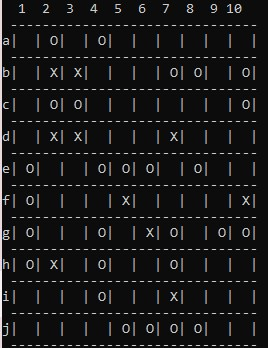
\includegraphics[width=0.45\textwidth]{HEL_template/figures/battleship.jpg}
    \caption{A player's game board during game play }
    \label{battleship game board}
\end{figure}

\section{Employed Tools and Technology}
The battleship game was designed using the C programming language on a laptop. The software used in writing the C language is CodeBlock. To achieve the goal of this project, several online tools were used. At first, because there was no initial knowledge of what a battleship game is, the use of YouTube to watch an in-depth explanatory of how to play a battleship game\cite{a2} was a.  great tool. Another tool used was Miro \cite{a3}. The online Miro white card dashboard was used for our brainwriting (brain-coding). The third tools used are the lecture slides from Professor Dr Tim Schattkowsky and Professor Dr Georg Birkenheuer. The fourth tool used is lucidchart\cite{a4}. Lucidchart is an online intelligent diagramming tool to draw UML diagrams. The UML diagram drew helped us make a better decision before coding. 

\section{Game Architecture (module structure)}
The figure below is an architecture of the battleship game. When the game starts, an audio sound will be played. This audio sound indicates the game is working; also, welcome graphics will be displayed. The next is user input, which will lead to the game's logic, then the game graphics and output displayed.

\begin{figure}[h]
    \centering
    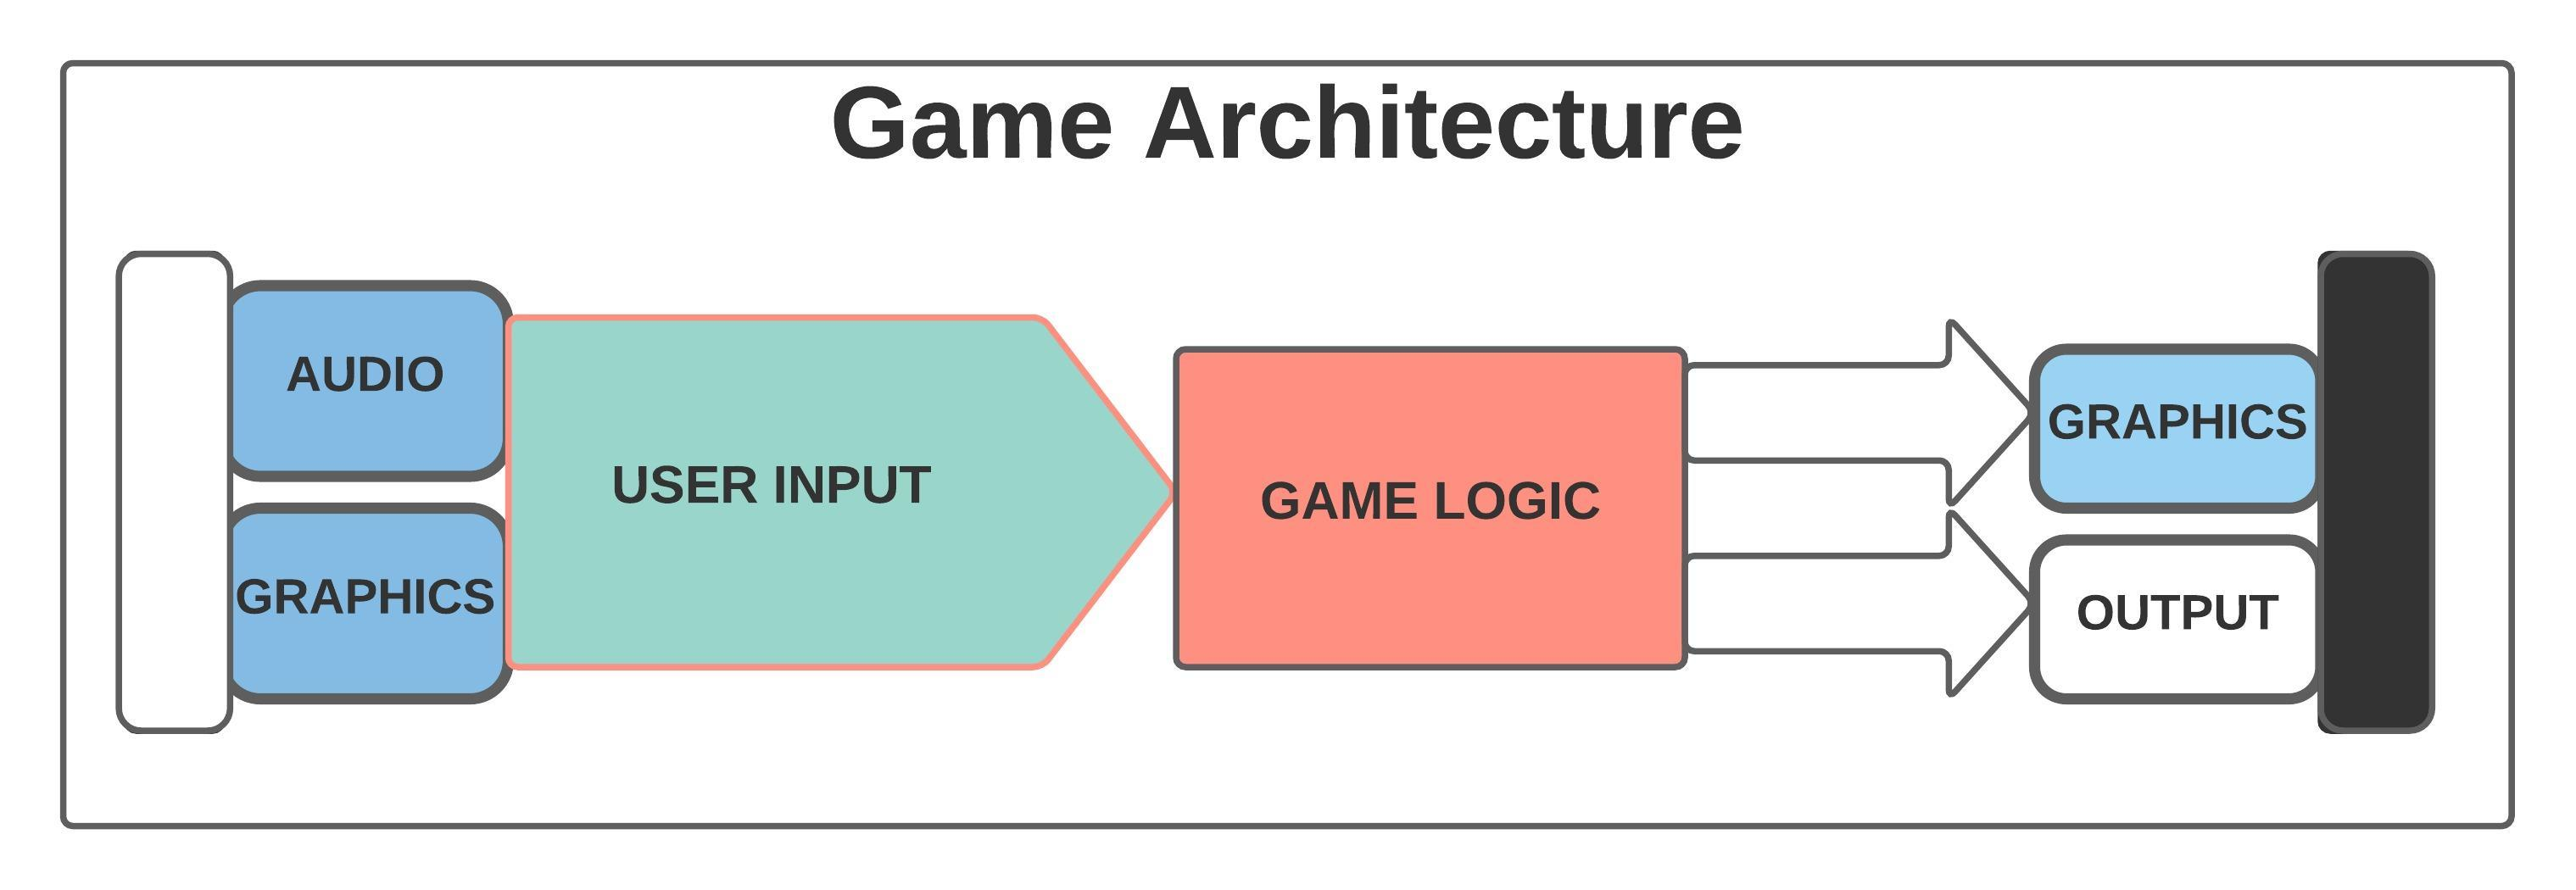
\includegraphics[width=0.72\textwidth]{HEL_template/figures/gameart.jpeg}
    \caption{The Game Architecture}
    \label{game architecture}
\end{figure}

\section{Major Design Decisions}
There are several decisions taken while designing the game. One of the decision is a simple user interface. Whenever the user is at any submenu, there is an option to go back to the previous menu instead of closing the game and starting all over. Another decision taken in designing the game is to place the ships manually. This is because the game is played on one PC, an opponent can memorize the placement of the other user. This will kill the fun of the game. For the sake of bragging right, whenever anyone plays against his friend, we have included a last played status menu that shows if the previous game played is a win/lose or a draw game. This idea is shown in the figure below.

\begin{figure}[h]
    \centering
    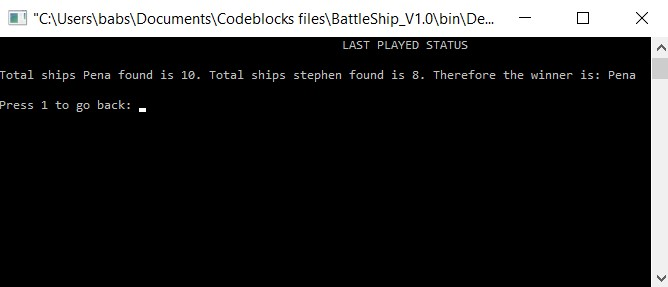
\includegraphics[width=0.98\textwidth]{HEL_template/figures/gameplaystatus.jpg}
    \caption{Last Played Status}
    \label{gamestatus}
\end{figure}

\begin{figure}[H]
    \centering
    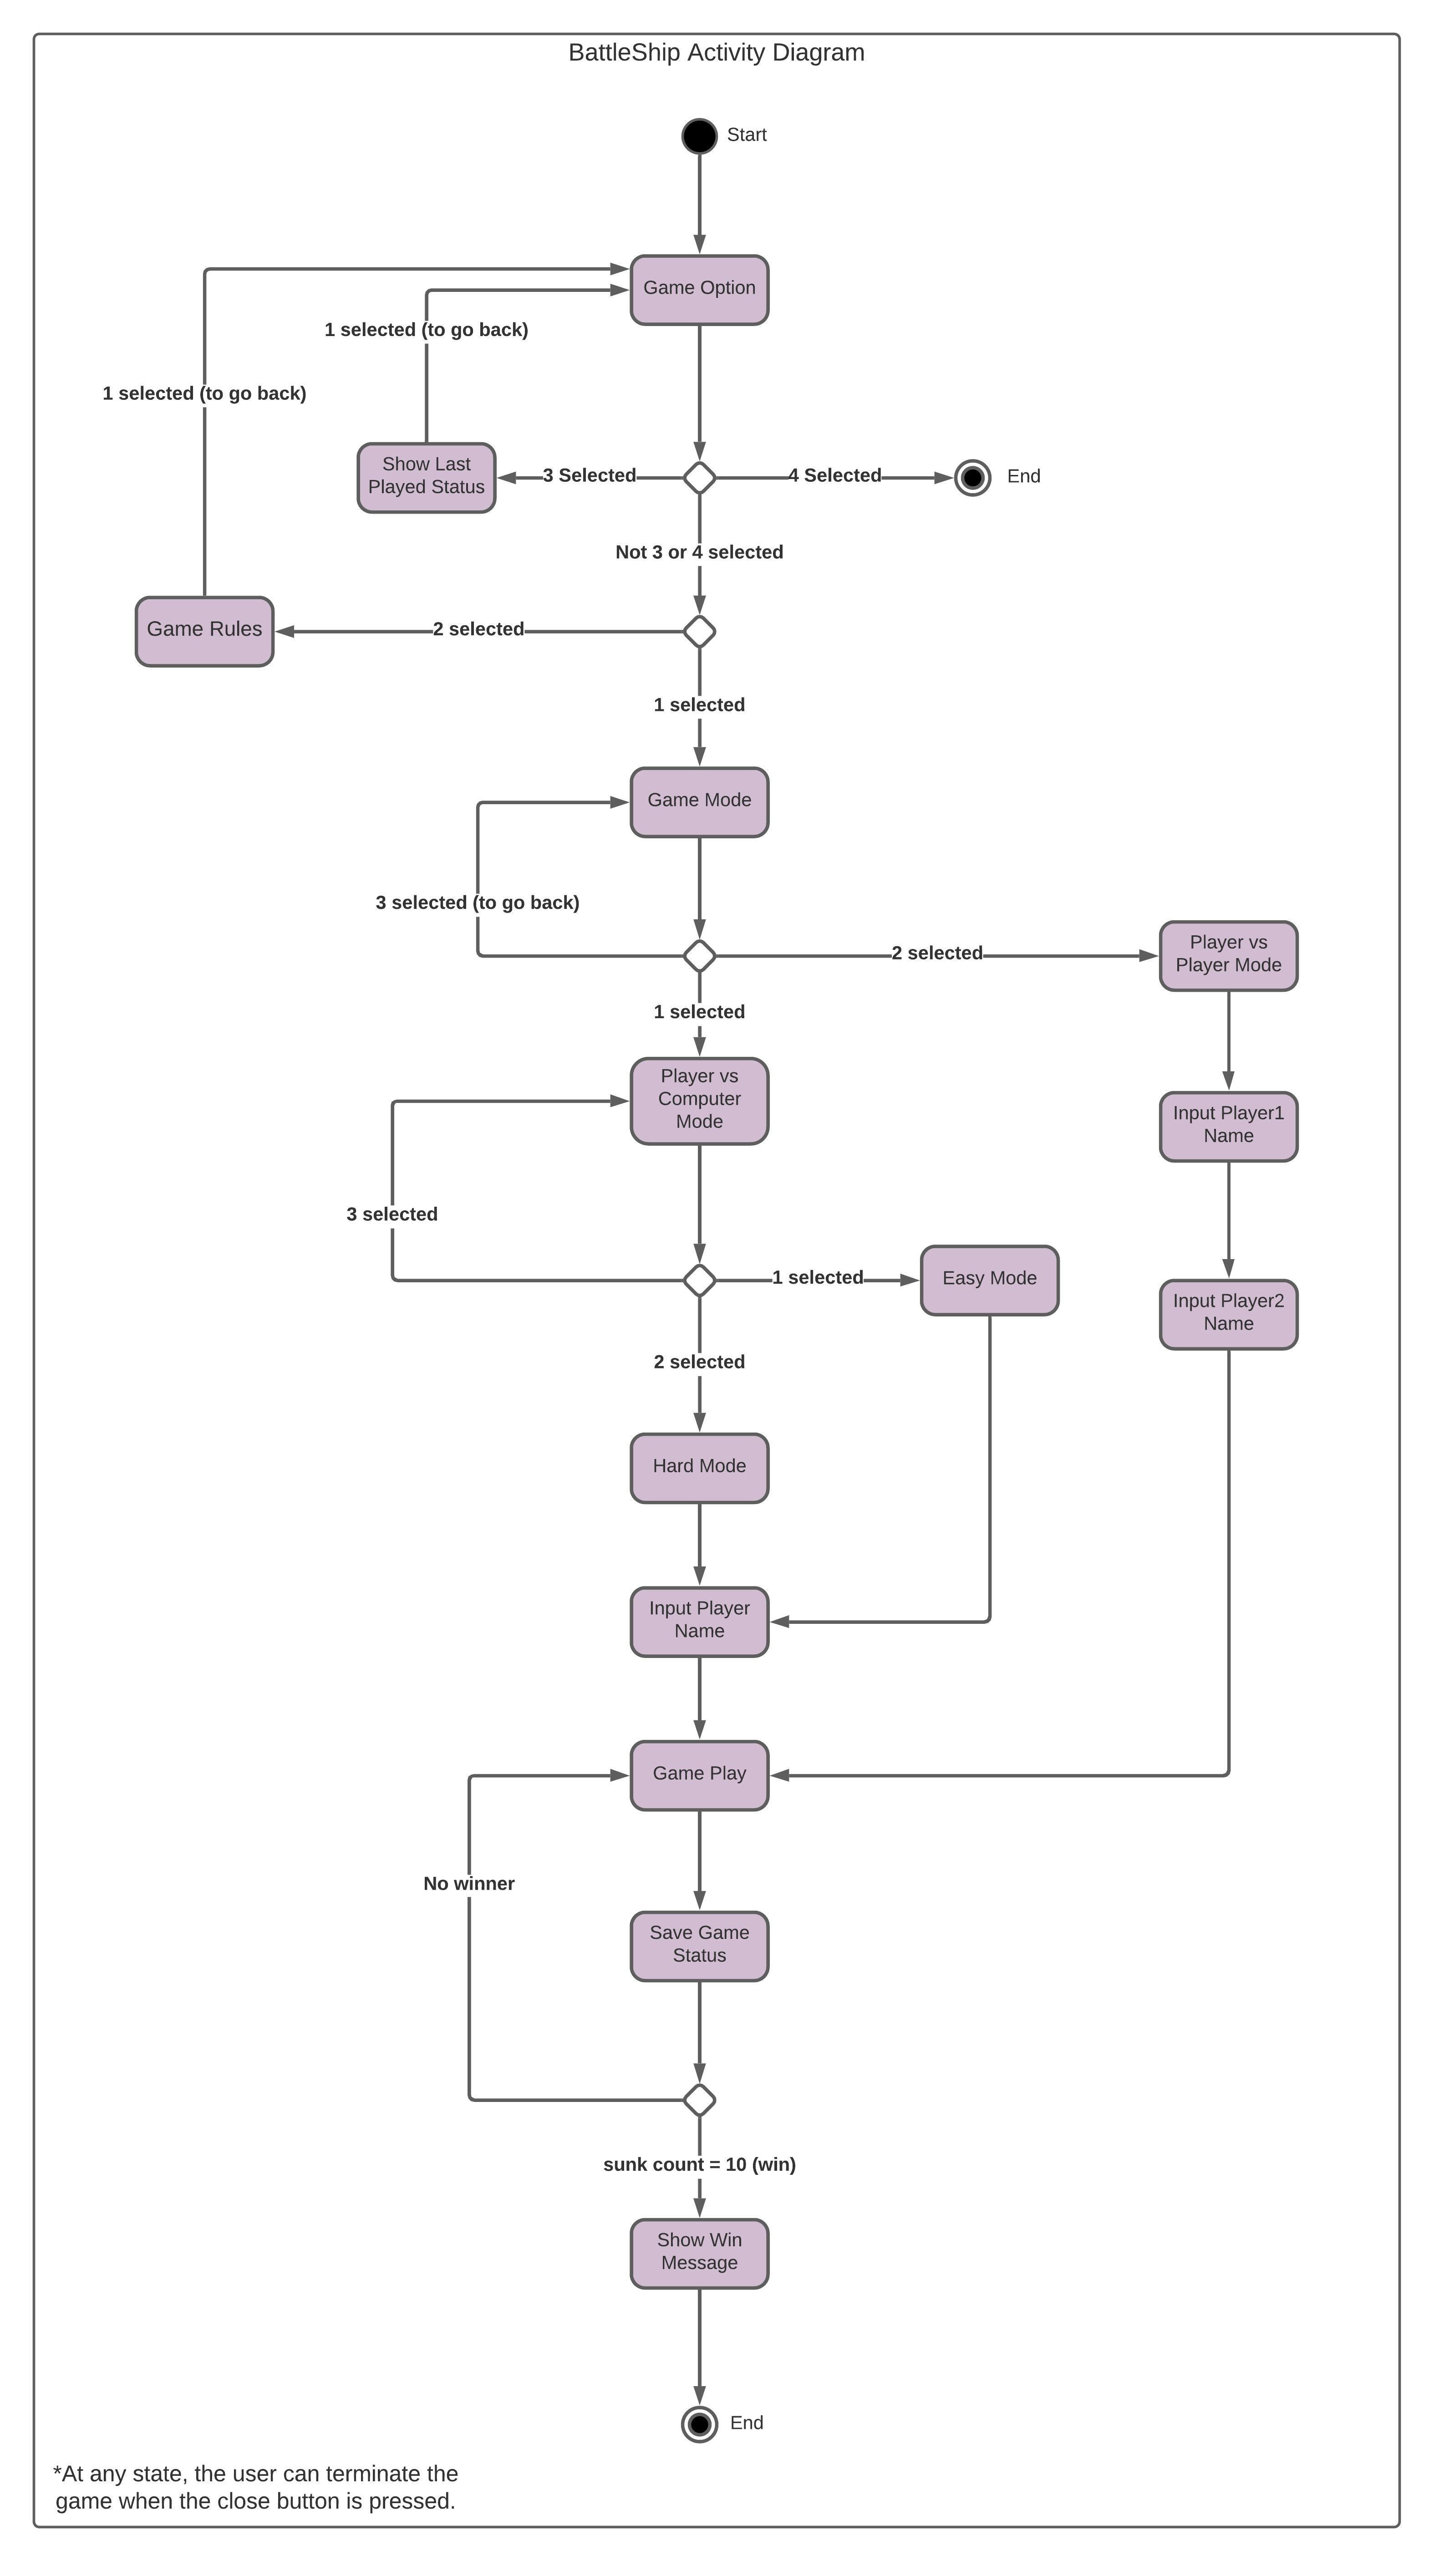
\includegraphics[width=0.85\textwidth]{HEL_template/figures/BattleS.jpeg}
    \caption{Battle-Ship Activity Diagram}
    \label{battleship1}
\end{figure}

\section{Game Implementation}
The battleship game runs in a sequential flow. This can be seen in figure 4. In general, when the game is started, the user has several options to select from. At any submenu, the user can go to the previous menu. The design of the game enables player vs player mode and player vs computer mode. If player vs computer is selected, there is also an option to choose an easy mode or hard mode. For easy mode, the computer guesses the positions of the ships randomly, while in hard mode, the computer will correctly sink seven ships of its opponent; thereafter, the play will be random. Whenever a ship has been sunk, there is a getstatus generated. The getstatus txt file generated will show how many ships has been sunk by a player.
In figure 5 below shows the activity diagram to set difficulty mode when playing against a computer. The logic is the use of switch case. In player vs computer mode, if the user enters 1, the mode is set to easy mode and if 2 is entered, the game is set to hard mode while 3 return the submenu to the previous menu.

\begin{figure}[H]
    \centering
    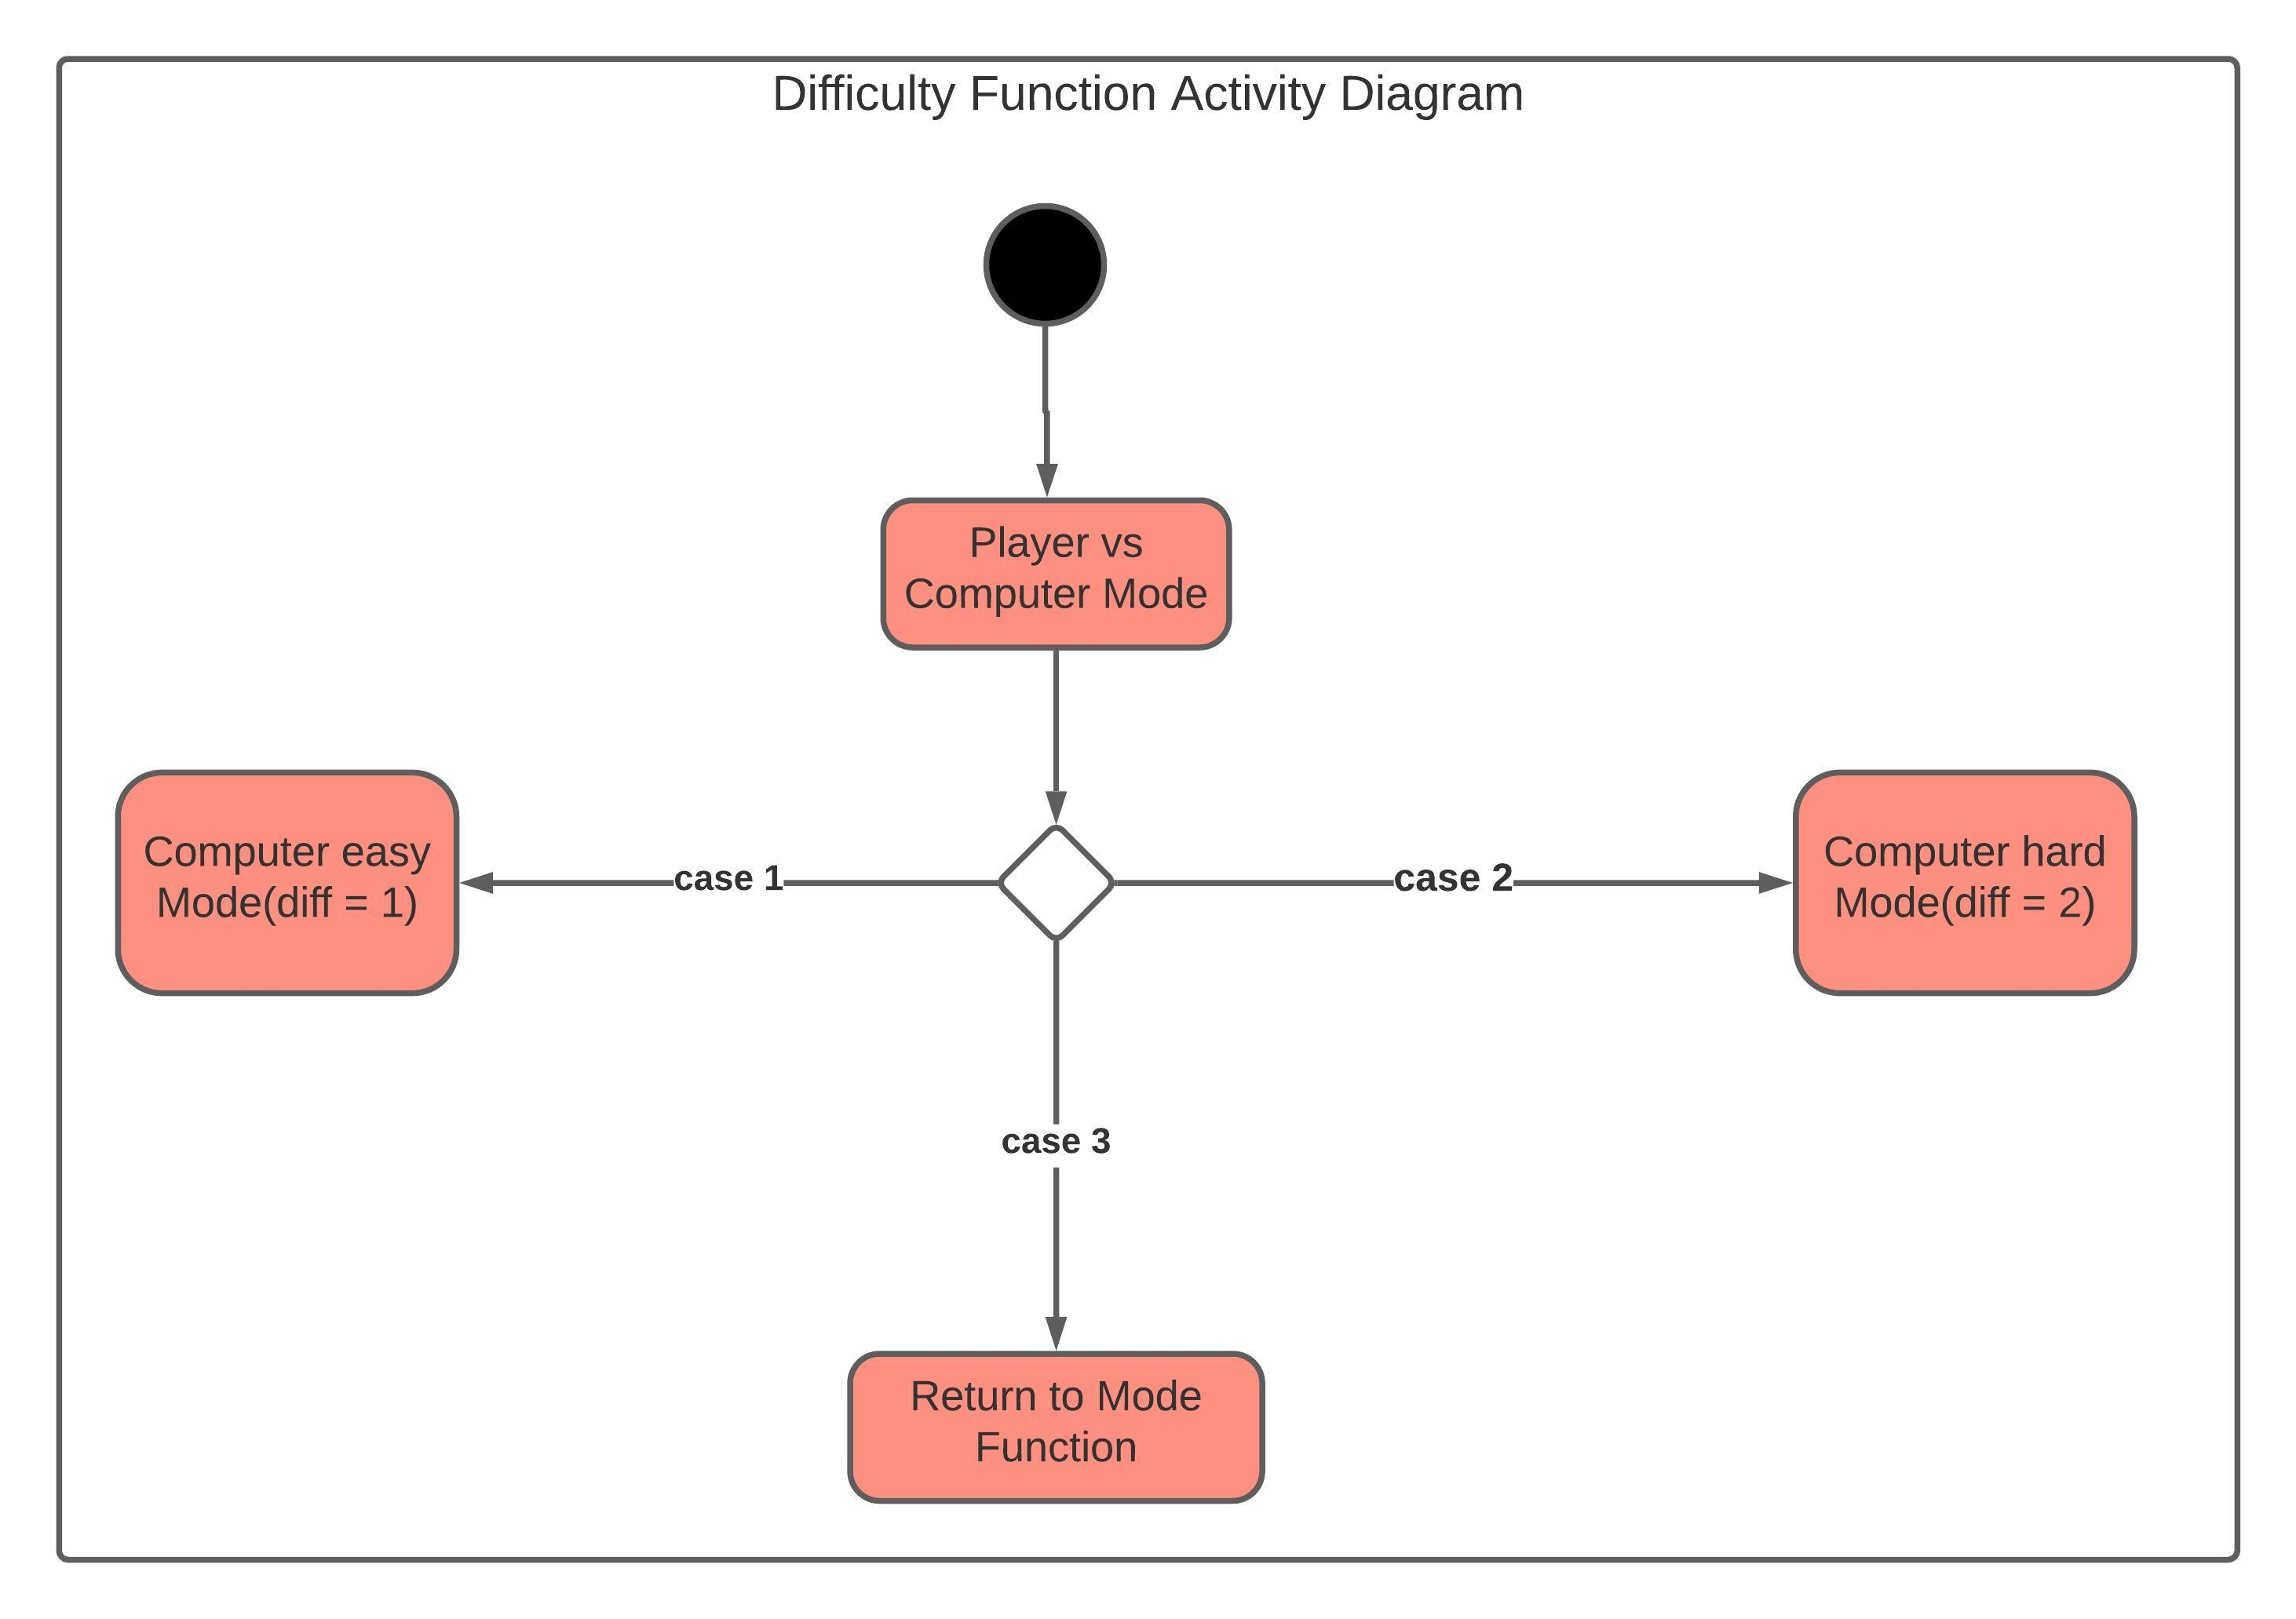
\includegraphics[width=0.98\textwidth]{HEL_template/figures/diff.jpeg}
    \caption{Activity Diagram for Difficulty Function}
    \label{difficulty}
\end{figure}

Figure 6 below is the activity diagram that shows how the game play function works. When in play mode, it will always be the player's turn to play at first and when there is a miss, the game switches to the next player (payer2 or computer) otherwise the player keeps playing until all ships are sunk.

\begin{figure}[H]
    \centering
    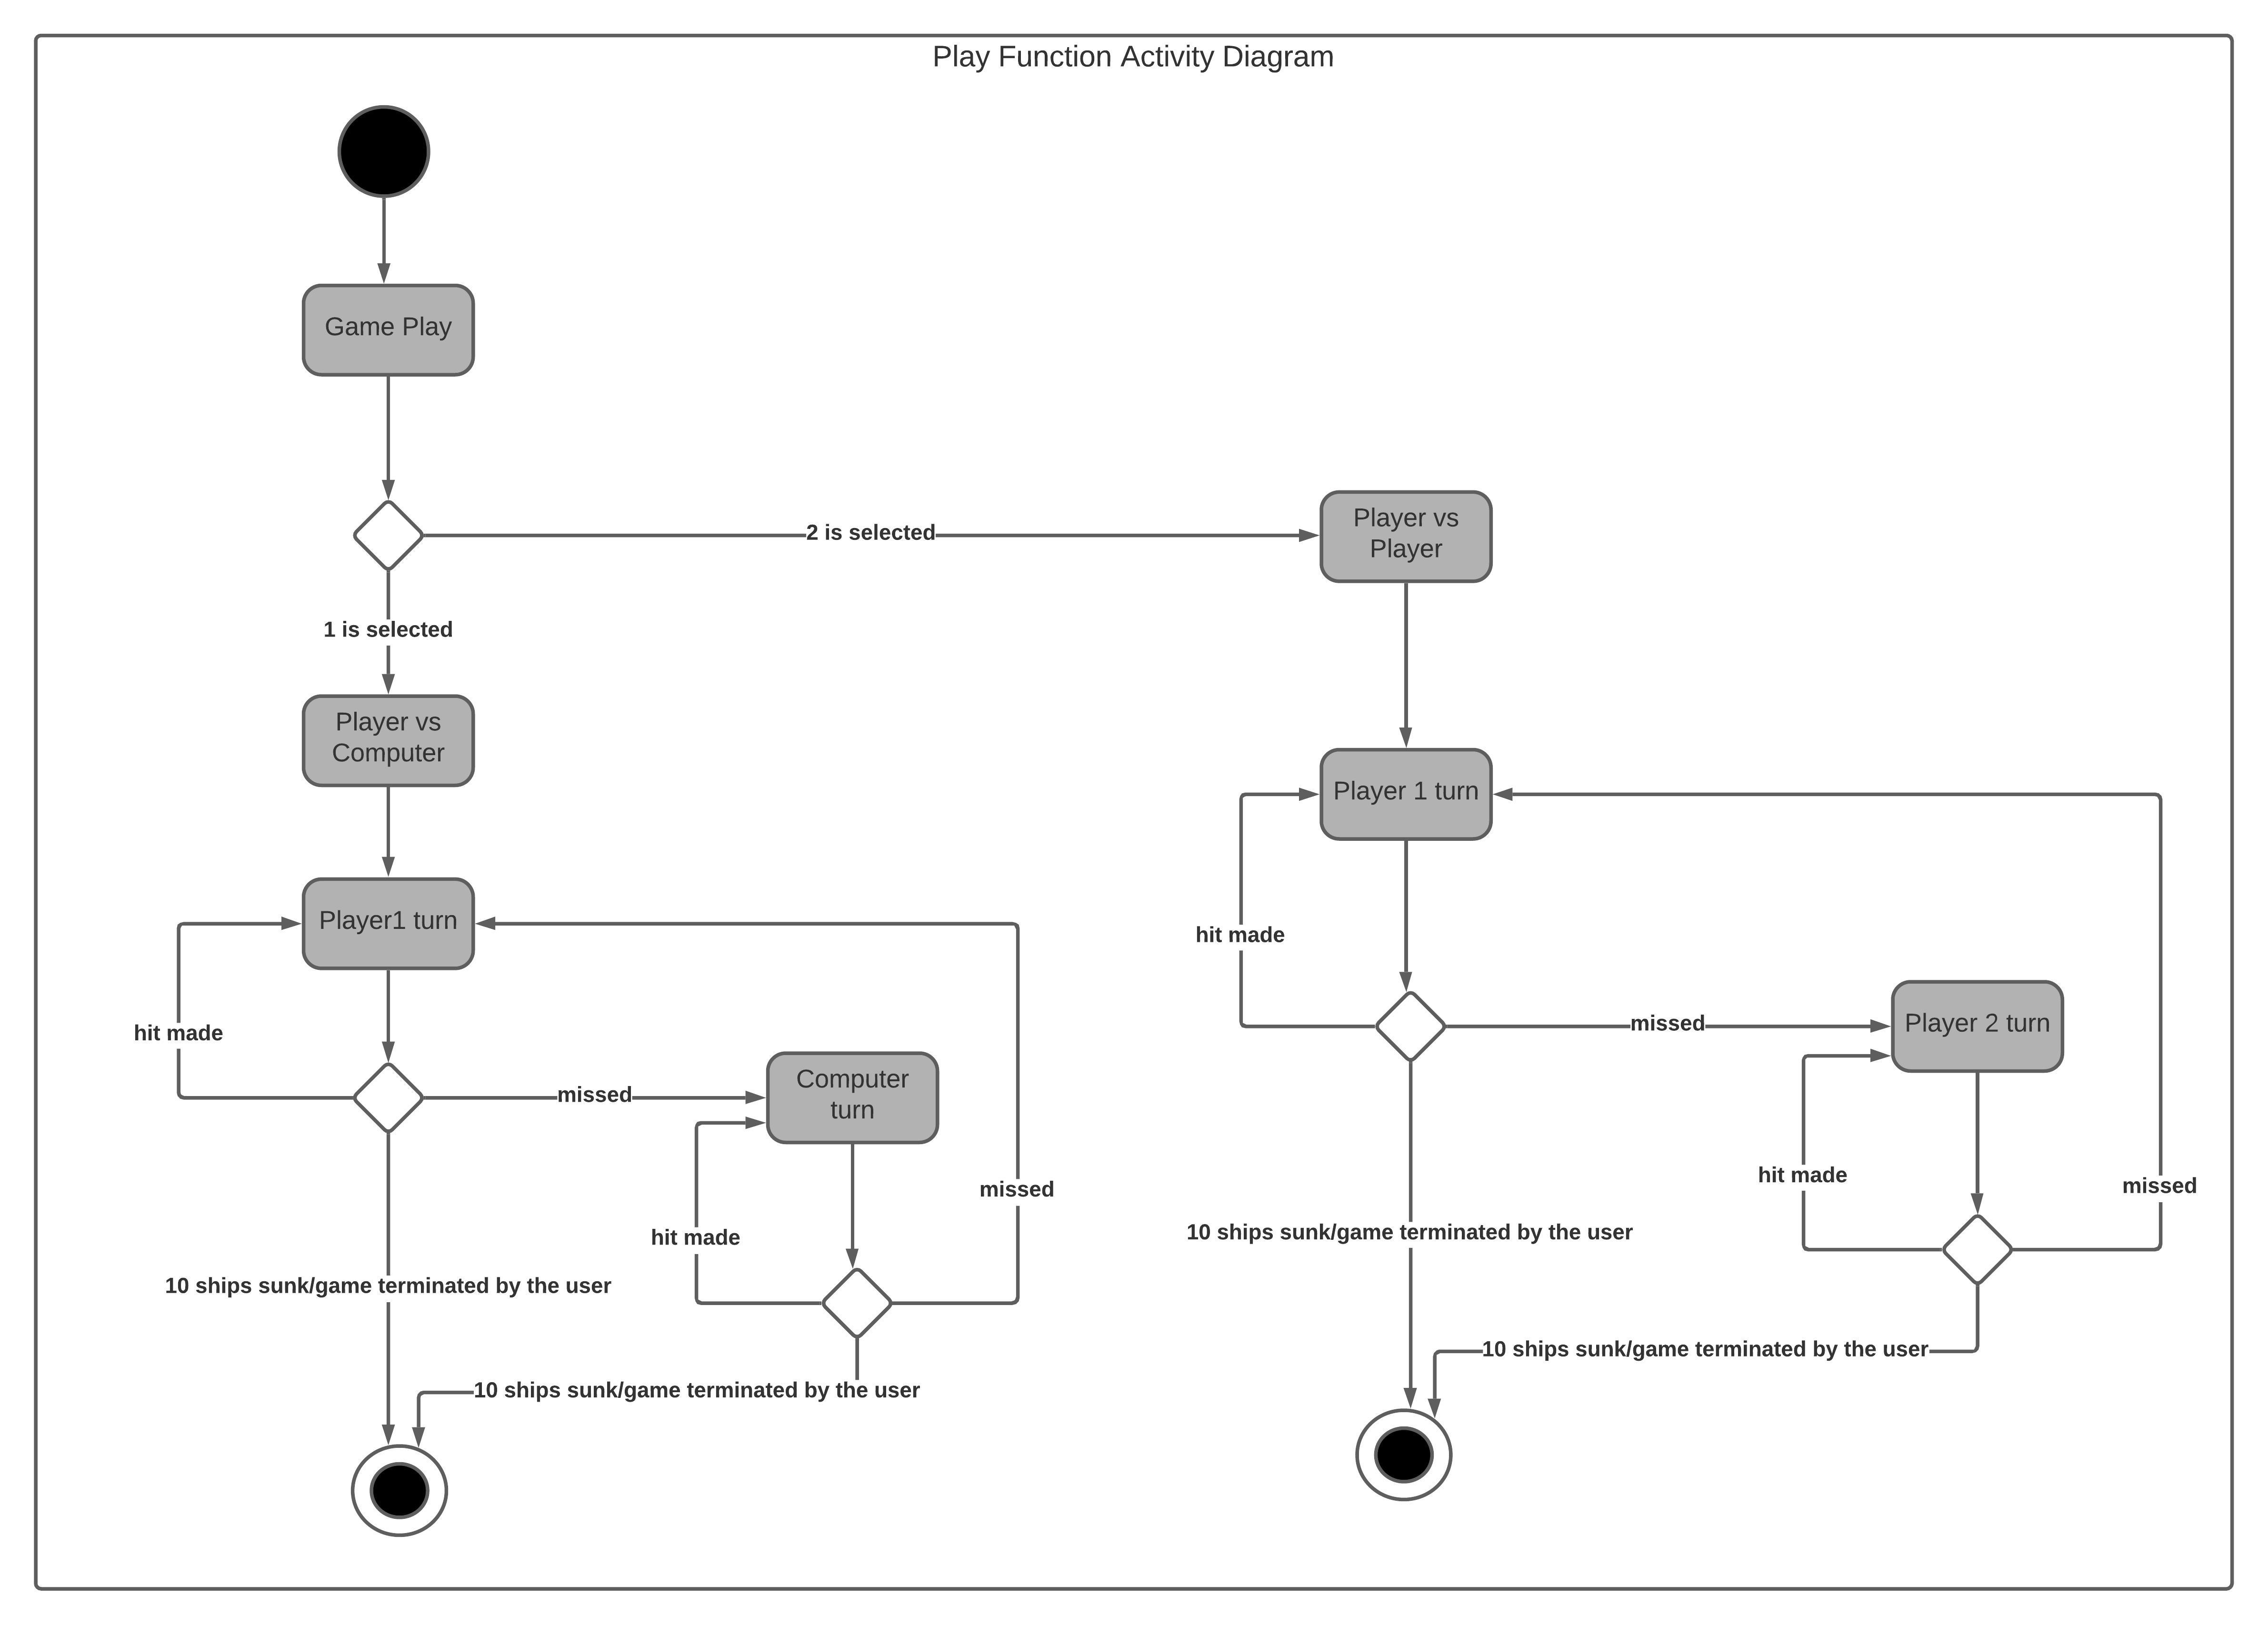
\includegraphics[width=0.68\textwidth]{HEL_template/figures/playf.jpeg}
    \caption{Activity Diagram for Play Function}
    \label{play}
\end{figure}

To check win, a variable called sunkcount1 and sunkcount2 has been initialized for both players. At first, these variable were set to zero. Whenever there is a ship sink, the variable updates its count. The player that gets to sunkcount = 10 wins the game. The logical flow can  be seen in figure 7 below.

\begin{figure}[H]
    \centering
    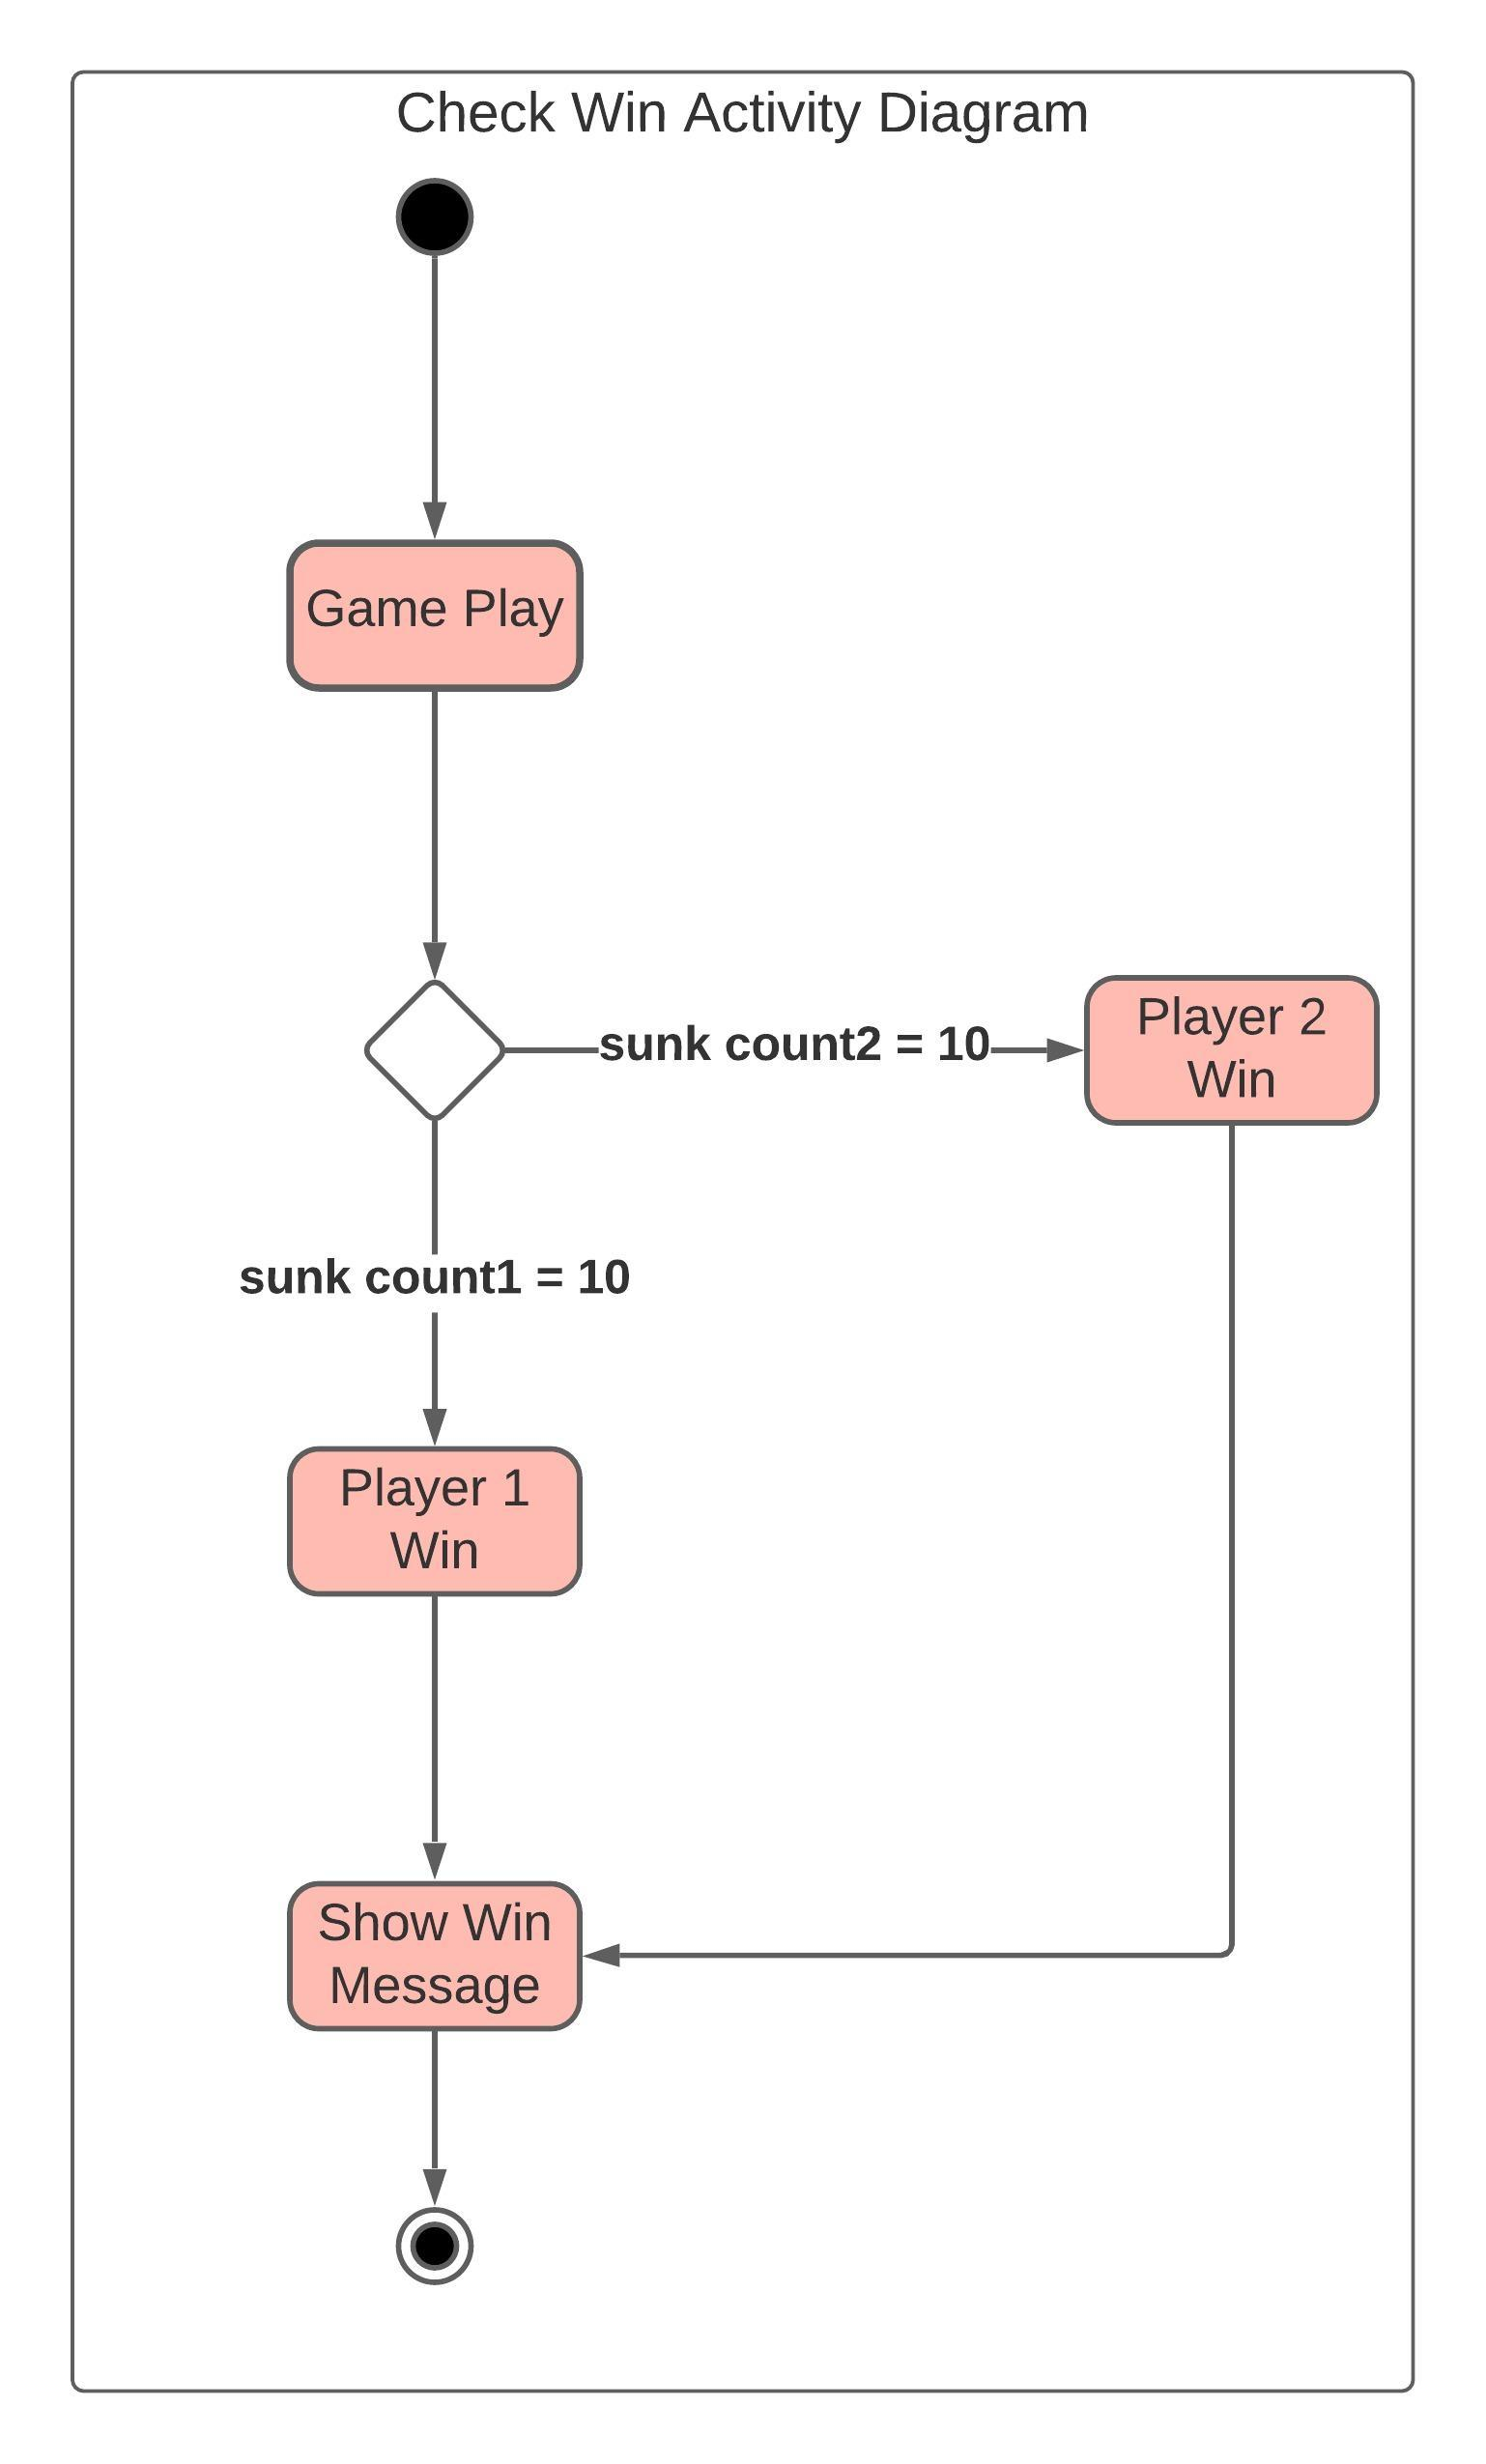
\includegraphics[width=0.48\textwidth]{HEL_template/figures/Checkwin.jpeg}
    \caption{Activity Diagram to Check-Win Function}
    \label{checkwin}
\end{figure}

There are two players who take turn in playing the game. Whenever any players misses a hit, it will be the next player's turn. This feature will occur automatically with the use of toggle function created. The activity diagram in figure 8 shows the flow logic when writing the code. At first, it will be player 1 turn. If there is a hit, player 1 will keep playing until there is a miss.

\begin{figure}[H]
    \centering
    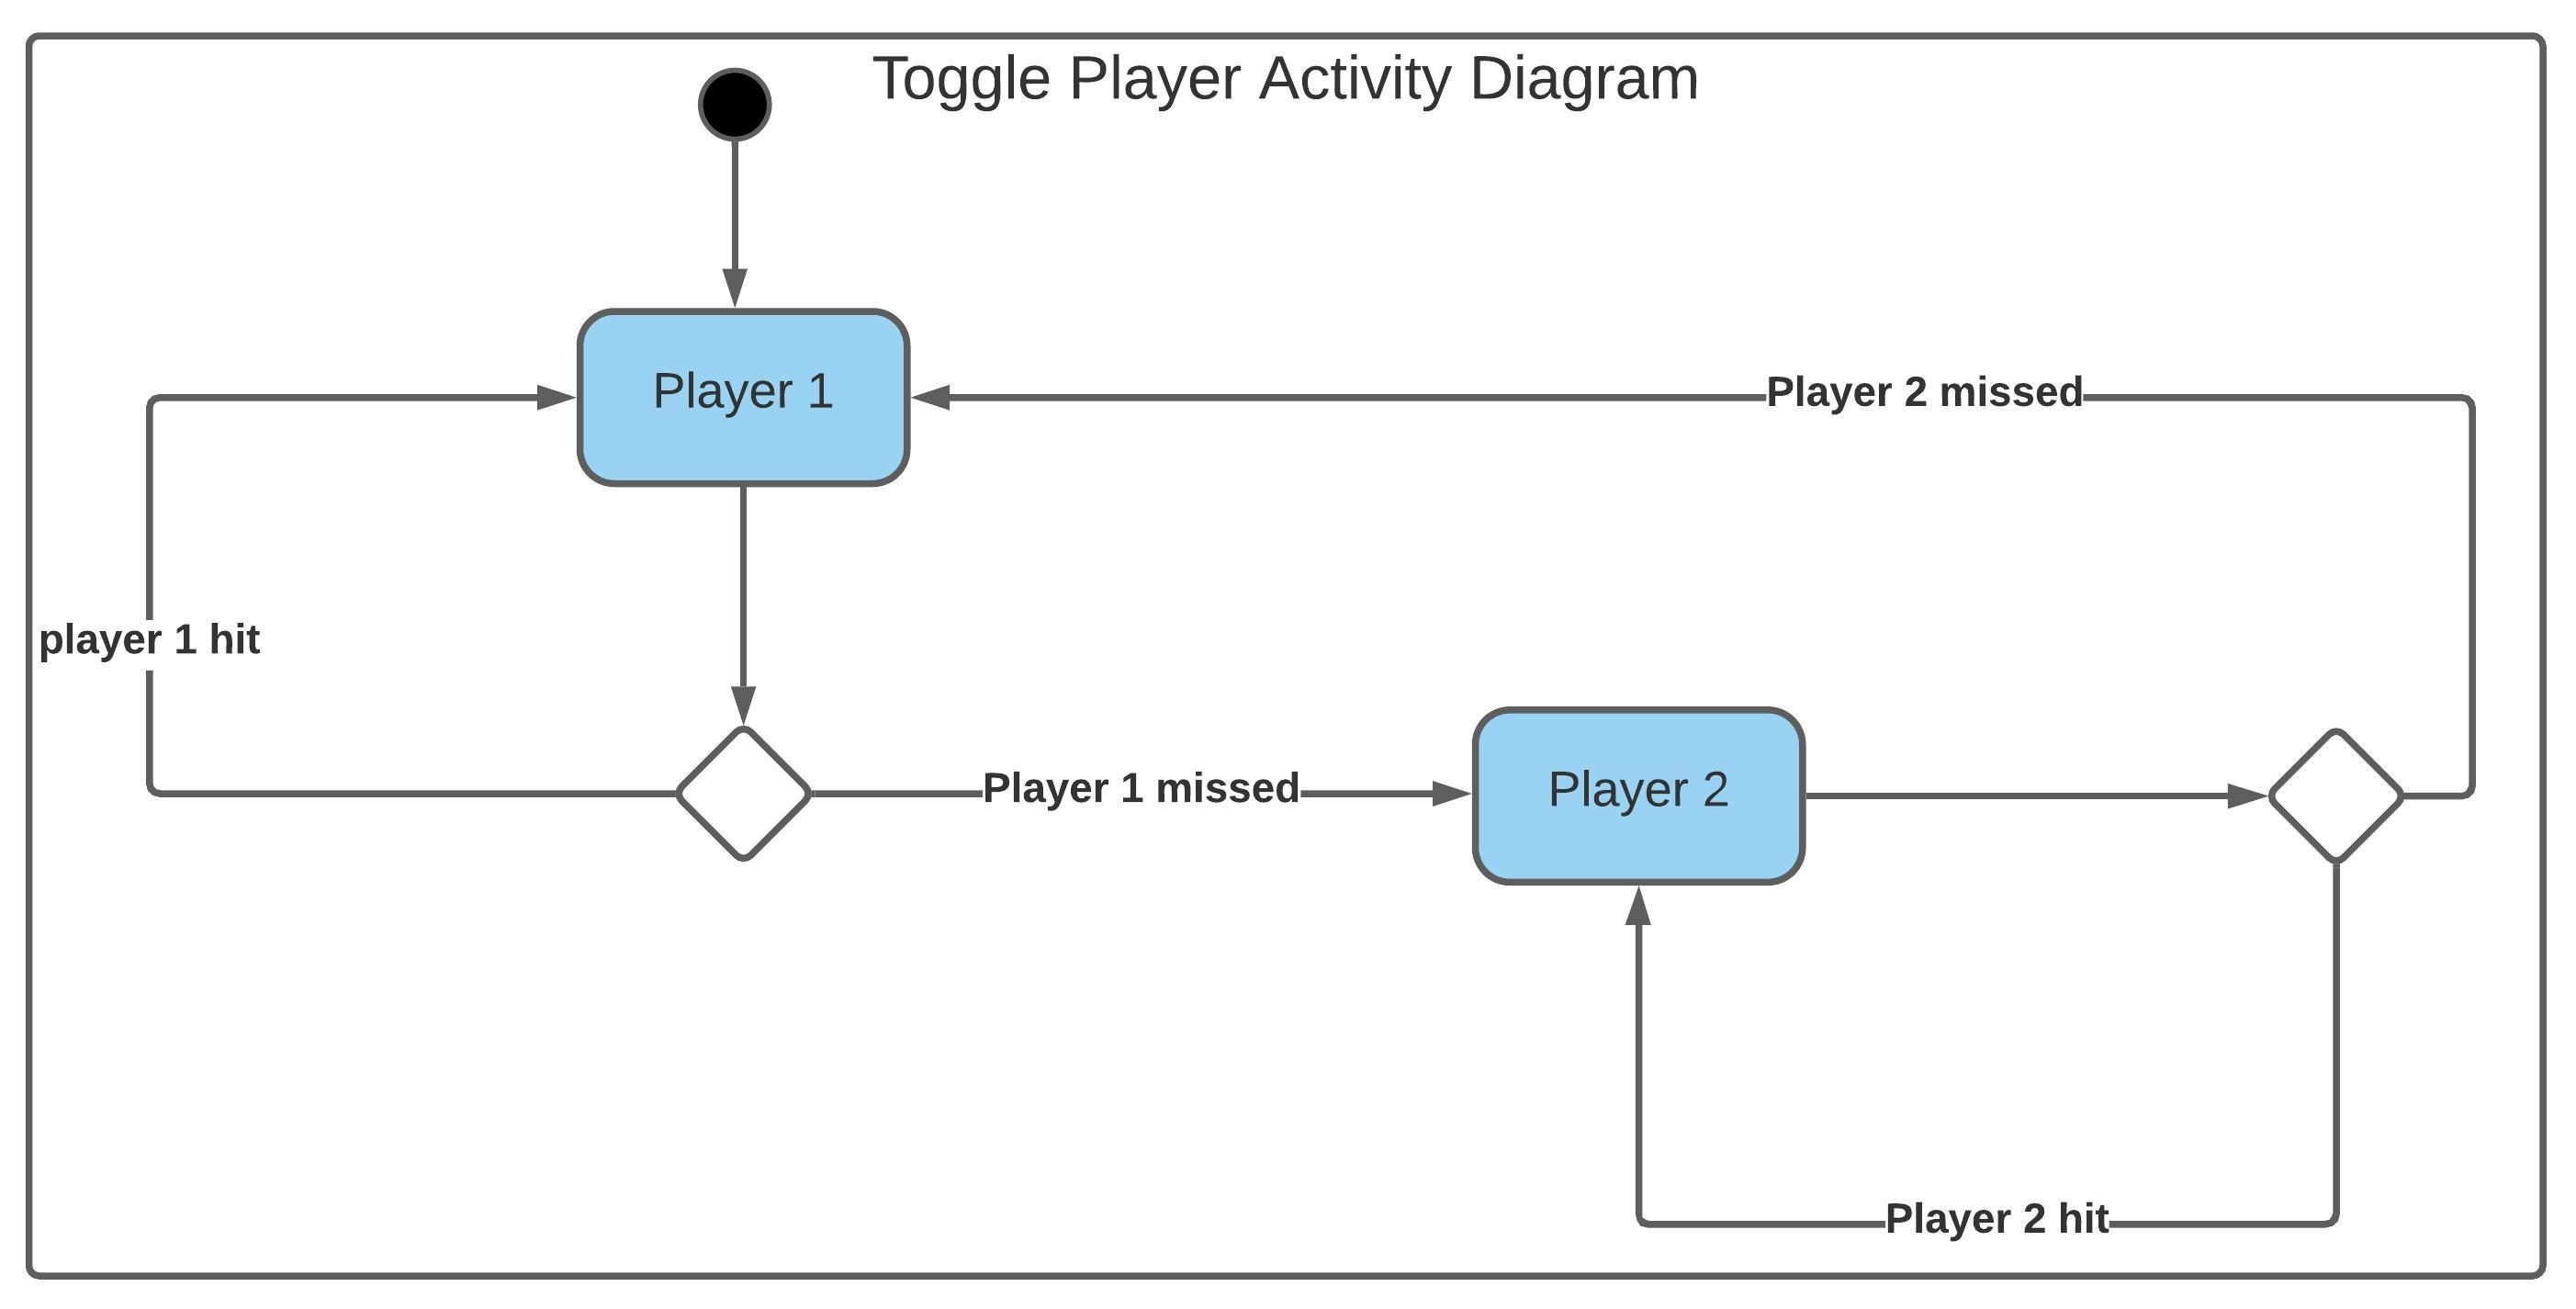
\includegraphics[width=0.88\textwidth]{HEL_template/figures/ToggleP.jpeg}
    \caption{Toggle Player Activity Diagram}
    \label{toggle}
\end{figure}

The battleship game requires that a player should guess correctly the position of his opponent ship and in that case, the ship will be sunk (destroyed). To achieve this, an activity diagram in figure 9 below shows the flow of how the code function work.

\begin{figure}[H]
    \centering
    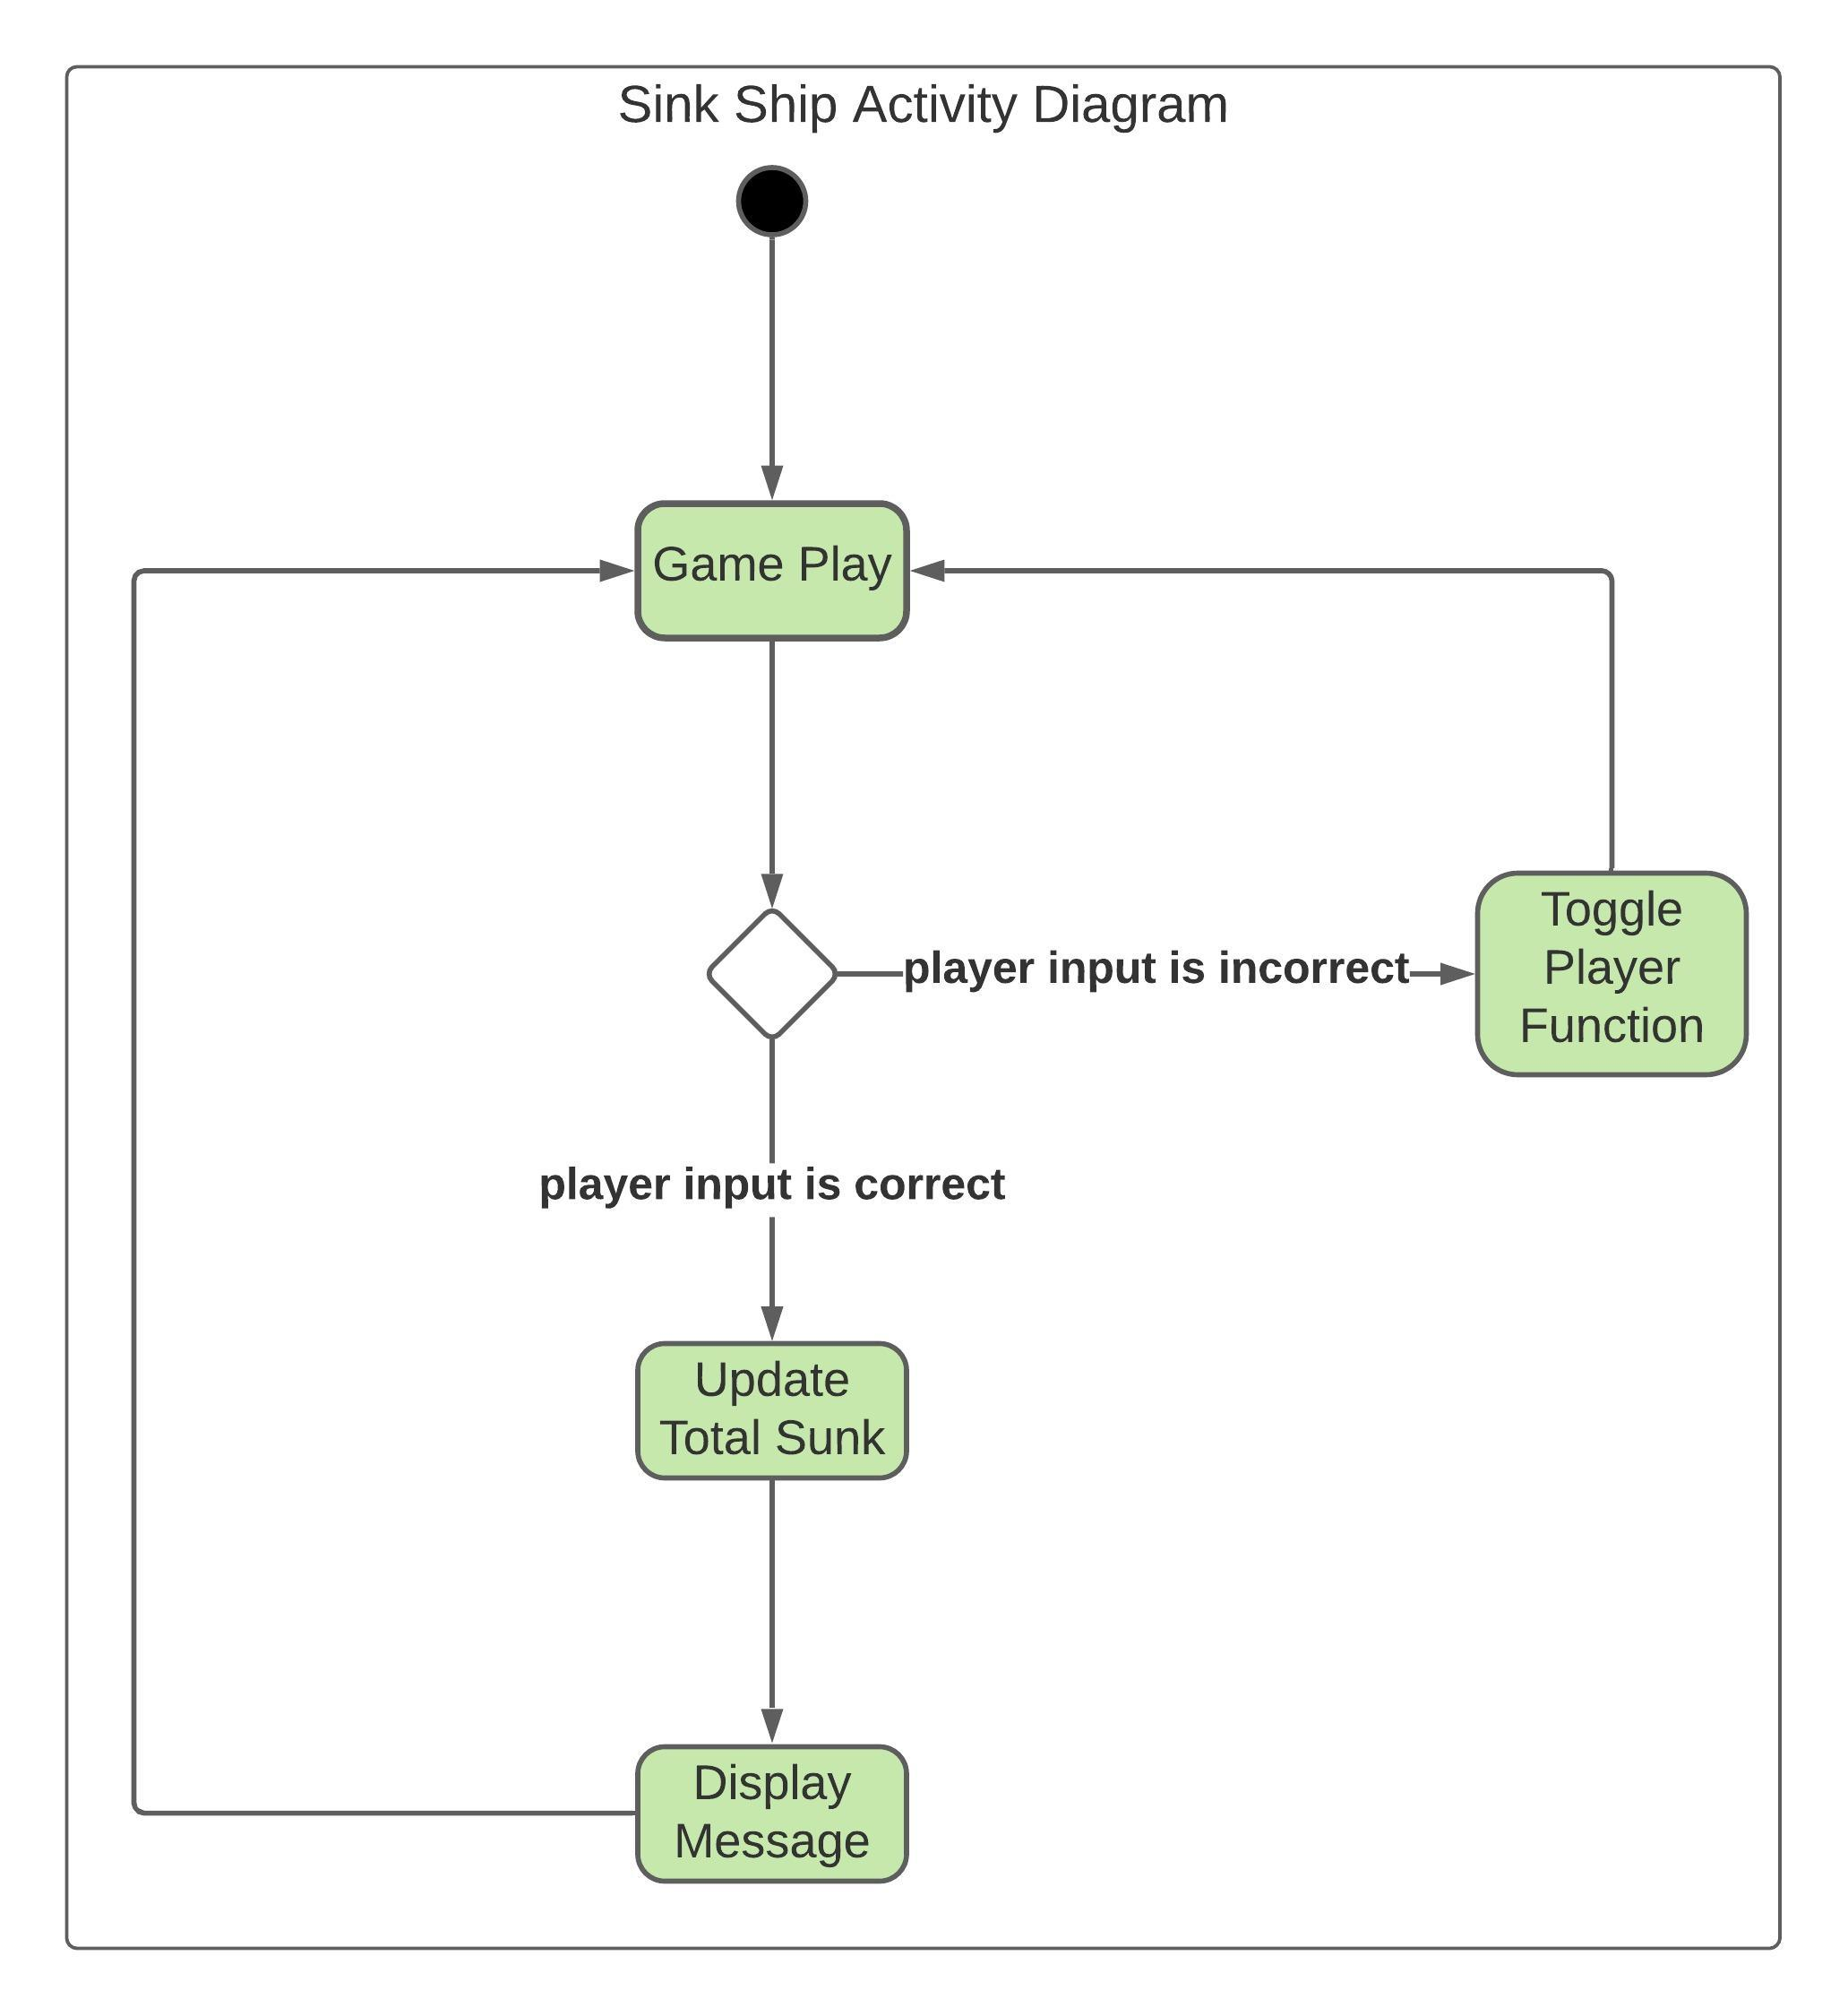
\includegraphics[width=0.68\textwidth]{HEL_template/figures/SinkShip.jpeg}
    \caption{Activity Diagram for Sink-Ship Function}
    \label{Sinkship}
\end{figure}

\section{Team Organisation}
The battleship game was developed and coded by Pena Benafa and Patrick Stephen. To achieve our goal, we met thrice in a week (Monday, Thursday and Friday) using about 4 hours in each day. We worked simultaneously in developing the game code so that there won't be any lapses.


\section{Conclusion}
There are various battleship game designed to be played on computer, therefore digitalizing the game. The game developed by the NG team has features such as can go back, can open game status, can play a sound. There are others features such as the ability to play online with a user on a different PC as well as a count-down timer to check player unnecessary delay will be added.

\newpage
\bibliographystyle{plain}
\bibliography{mybibfile}

\clearpage
\pagenumbering{arabic}% resets `page` counter to 1
\renewcommand*{\thepage}{A\arabic{page}}
\end{document}
